%%%%%%%%%%%%%%%%%%%%%%%%%%%%%%%%%%%%%%%
%Created by Yuan Kaixin
%Run with XeLaTeX, 
%then BibTeX, 
%then XeLaTeX, 
%then XeLaTeX
%%%%%%%%%%%%%%%%%%%%%%%%%%%%%%%%%%%%%%%


\documentclass[12pt]{article}%normal字体为12磅,也即小四

%%%%%%%%%%%%%%%%%%%%%%%%%%%%%%%
%Packages
%%%%%%%%%%%%%%%%%%%%%%%%%%%%%%%
\usepackage{indentfirst}	%引用这一宏包,每段段首自动缩进
\usepackage{amsmath}		%公式环境宏包,最好不要取消
\usepackage{xeCJK}			%中日韩语环境宏包,只能用xelatex编译,不能用pdflatex编译
\usepackage{graphicx}		%图片环境
%\usepackage{verbatim}		%代码块宏包,如果报告中需要插入代码,则需要此宏包,反之,可以注释掉此宏包以节省编译时间
\usepackage{float}				%图片浮动体环境,存在这一宏包,图片位置可以通过[H]句柄固定
\usepackage{hyperref}		%超链接环境,引用这一宏包,图片公式等可以交叉引用跳转。
%\usepackage{authblk}			%作者区环境,如不需要生成类似论文中的作者信息区,则不需要此宏包
\usepackage[round]{natbib}%人名-时间引用文献格式,round句柄表示外围为圆括号
%\usepackage{multicol}		%多栏排版格式宏包,例如两栏文字,三栏文字等。具体使用方法见multicol的帮助文档
\usepackage[hmargin=1.25in, vmargin=1in]{geometry}%A4格式标准页边距
\usepackage{CJKpunct}	%中日韩语标点符号
\usepackage{fancyhdr}		%页眉页脚环境,用于生成页码
\usepackage{lastpage}		%尾页的引用宏包,用于配合fancyhdr宏包
\usepackage{array}				%高级表格环境宏包
\usepackage[normalem]{ulem}				%智能下划线环境,句柄normalem取消了宏包与\emph标志的绑定,最好不要更改,否则会影响参考文献等默认使用\emph的部分。
\usepackage{color}				%颜色支持宏包。不需要带有色彩的字体,则注释此项。图片不受影响。
\usepackage{fontawesome}	%矢量图小图标宏包。通常来说用不到,你可以直接注释掉。

%%%%%%%%%%%%%%%%%%%%%%%%%%%%%%%
%杂项
%%%%%%%%%%%%%%%%%%%%%%%%%%%%%%%
\hypersetup{colorlinks={false}}%超链接有无颜色,false为无。
\punctstyle{banjiao}%半角标点符号
\bibliographystyle{plainnat}%参考文献引用样式

%%%%%%%%%%%%%%%%%%%%%%%%%%%%%%%
%Fonts
%%%%%%%%%%%%%%%%%%%%%%%%%%%%%%%
\setmainfont{Times New Roman}%英文字体
\setCJKmainfont[AutoFakeBold={2.17}, AutoFakeSlant={0.3}]{宋体}%中文字体
\xeCJKsetup{CJKmath = true}%公式可用中日韩语
%\xeCJKsetup{AutoFakeBold = {2.17}}

%%文中可能用到的字体和行距
\newcommand{\Biaoti}{\fontsize{26pt}{36pt}\selectfont}           % 一号, 1.4 倍行距
\newcommand{\xiaosan}{\fontsize{15pt}{5pt}\selectfont}        % 小三, 表格专用
\newcommand{\Xiaosan}{\fontsize{15pt}{30pt}\selectfont}        % 小三,单倍行距
\newcommand{\xiaosi}{\fontsize{12pt}{18pt}\selectfont}            % 小四, 1.5倍行距
\newcommand{\lastthing}{\fontsize{12pt}{15pt}\selectfont}

%%%%%%%%%%%%%%%%%%%%%%%%%%%%%%%
%浮体、编号等名称重定义
%%%%%%%%%%%%%%%%%%%%%%%%%%%%%%%
\renewcommand\contentsname{目录}
\renewcommand\partname{}
\renewcommand\appendixname{附录}
\renewcommand\refname{\Xiaosan\textbf{参考文献}}
%\renewcommand\Authands{ , }
\renewcommand\figurename{图}

%%%%%%%%%%%%%%%%%%%%%%%%%%%%%%%
%页脚样式
%%%%%%%%%%%%%%%%%%%%%%%%%%%%%%%
\pagestyle{fancy}
\fancyhf{}
\fancyfoot[C]{第\ \thepage\ 页,共\ \pageref{LastPage}\ 页}
\renewcommand{\headrulewidth}{0pt}

%%%%%%%%%%%%%%%%%%%%%%%%%%%%%%%%%%%%%%%%%
%样式设置区
%%%%%%%%%%%%%%%%%%%%%%%%%%%%%%%%%%%%%%%%%
\newcommand{\reposec}[1]{\section{\Xiaosan\textbf{#1}}}
\newcommand{\reposubsec}[1]{\subsection{\xiaosi\textbf{#1}}}

%%%%%%%%%%%%%%%%%%%%%%%%%%%%%%%%%%%%%%%%%
%封面信息区
%必须反复核实!
%%%%%%%%%%%%%%%%%%%%%%%%%%%%%%%%%%%%%%%%%
\newcommand{\reportuse}{研究生学位论文中期报告}%报告用途
\newcommand{\reponame}{基于非晶合金材料的磁通门磁强计设计}%报告题目
\newcommand{\authname}{袁恺鑫}                                               %%%%%%%作者
\newcommand{\authnumb}{201918007513012}%学号
\newcommand{\teacname}{杜爱民}%老师
\newcommand{\teachrank}{研究员}%职称
\newcommand{\studerank}{理学博士}%学位类别
\newcommand{\majorarea}{地球与空间探测技术}%学科专业
\newcommand{\majorproj}{空间物理探测技术}%研究方向
\newcommand{\instidepar}{中国科学院地质与地球物理研究所}%研究所(院系)
\newcommand{\datetable}{2022年1月5日}%填表日期

%%%%%%%%%%%%%%%%%%%%%%%%%%%%%%%%%%%%%%%%%
%标题信息区
%开题报告并不需要此项,因此全部注释
%%%%%%%%%%%%%%%%%%%%%%%%%%%%%%%%%%%%%%%%%
%\newcommand{\addcode}{北京\ 100029}%单位地点,邮编
%\title{\reponame}%制作标题
%\author[1]{\authname}%制作作者名
%\affil[1]{\instidepar,\addcode}%制作单位信息
%\date{}%制作写作日期,default:编译当天

%%%%%%%%%%%%%%%%%%%%%%%%%%%%%%%%%%%%%%%%%
%begin the document
%%%%%%%%%%%%%%%%%%%%%%%%%%%%%%%%%%%%%%%%%
\begin{document}
%%%%%%%%%%%%%%%%%%%%%%%%%%%%%%%%
%Head Matters
%\include{preface}%If the `prefacepro' below won't work properly, enable this file and edit it yourself
\thispagestyle{empty}%取消这一页的页码
%%%%%%%%%%%%%%%%%%%%%%%%%%%%%%%%
%Coded by Yuan Kaixin
%Unless Necessary, Don't edit this File!
%%%%%%%%%%%%%%%%%%%%%%%%%%%%%%%%
{\Large\ \par\ \par\ \par}
\begin{figure}[H]
\center

\includegraphics[width=12.81cm]{PICS/UCAS_Logo_Long.png}
\end{figure}
%\vspace{0.01cm}\par
\begin{center}
\noindent\Biaoti\textbf{\reportuse}\par
%{\textbf 研究生学位论文开题报告}
\vspace{6.5cm}
%\noindent\xiaosan\textbf{报告题目\uline{\ \ \reponame\ }}\\[2pt]
\xiaosan\bfseries
\begin{tabular}{p{60pt}>{\centering\arraybackslash}p{120pt}>{\centering\arraybackslash}p{30pt}>{\centering\arraybackslash}p{120pt}}
	报告题目&\multicolumn{3}{>{\centering\arraybackslash}p{275pt}}{\reponame}	\\ \cline{2-4}
	\ &\ &\ &\ \\[10pt]
	学生姓名&\authname&学号&\authnumb		\\ \cline{2-2}\cline{4-4}
	\ &\ &\ &\ \\[10pt]
	指导教师&\teacname&职称&\teachrank		\\ \cline{2-2}\cline{4-4}
	\ &\ &\ &\ \\[10pt]
	学位类别&\multicolumn{3}{>{\centering\arraybackslash}p{275pt}}{\studerank}	\\ \cline{2-4}
	\ &\ &\ &\ \\[10pt]
	学科专业&\multicolumn{3}{>{\centering\arraybackslash}p{275pt}}{\majorarea}	\\ \cline{2-4}
	\ &\ &\ &\ \\[10pt]
	研究方向&\multicolumn{3}{>{\centering\arraybackslash}p{275pt}}{\majorproj}	\\ \cline{2-4}
	\ &\ &\ &\ \\[10pt]
\end{tabular}
\begin{tabular}{p{95pt}>{\centering\arraybackslash}p{260pt}}
	研究所(院系)&\instidepar	\\ \cline{2-2}
	\ &\ \\[10pt]
\end{tabular}
\begin{tabular}{p{60pt}>{\centering\arraybackslash}p{295pt}}
	填表日期&\datetable	\\ \cline{2-2}
\end{tabular}\\
\Xiaosan\bfseries
\ \vspace{10pt}\\
中国科学院大学制
%Actually, It is made by Yuan Kaixin, Haha!
\end{center}%封面,此文件通常不需要修改

%If a CONTENT is needed, enable it below.
\thispagestyle{empty}%取消这一页的页码
\tableofcontents		%生成目录
\newpage        		%更换空白页

%制作标题行,可选,与导言中的标题信息区必须同时注释或反注释!
%\maketitle


%%%%%%%%%%%%%%
%Main Matter
%edit it yourself!
%there is a demo here!
%如果需要分页开始,则用\include{$CHAPTER}来包含相应的子文件
%如果不需要空白页,则用\input{$CHAPTER}包含。
%%%%%%%%%%%%%%
\xiaosi	%进入正文字体,具体见上
\setcounter{page}{1}%将这一页设定为第一页
\reposec{如何编写正文,正文子标题}
使用$\backslash reposec\{$ 填入节标题$\}$标志,生成正文的一个节标题。\par
正文每段文字直接书写,用$\backslash textbf\{$加粗$\}$来形成\textbf{加粗},$\backslash textit\{$斜体$\}$来形成\textit{斜体},$\backslash uline\{$下划线$\}$来形成\uline{下划线}。\par
在正文每段后采用$\backslash par$来分段,如此的话下一段会自动缩进。如果不希望分段,只是希望新启一行,那么只需要使用$\backslash\backslash$。\par
\reposubsec{正文子子标题}
使用$\backslash reposubsec\{$ 填入子节标题$\}$,生成正文的一个子节标题。\par
\paragraph{段标题}使用$\backslash paragraph\{$段标题$\}$起一段以此为段标题的新段落。这个段标题不参与缩进。\par%input命令可以嵌套调用,即每个被input的文件里,还可以用input来调用另一个文件。这样可以避免单个tex文件过长而不便于阅读。
\reposec{如何插入图片}
编译之后,右键点击图片,选择跳至原文件,查看更多关于插入图片的注释。参见下图\ref{fig00}。\par
\begin{figure}[H]%开启插图环境,句柄[H]为图片锁定在插入的位置,不进行灵活调整
\label{fig00}%图片引用标志,可以通过ref指令交叉引用,在全文内任意位置都可链接到此处。见上文。
\centering%图片居中
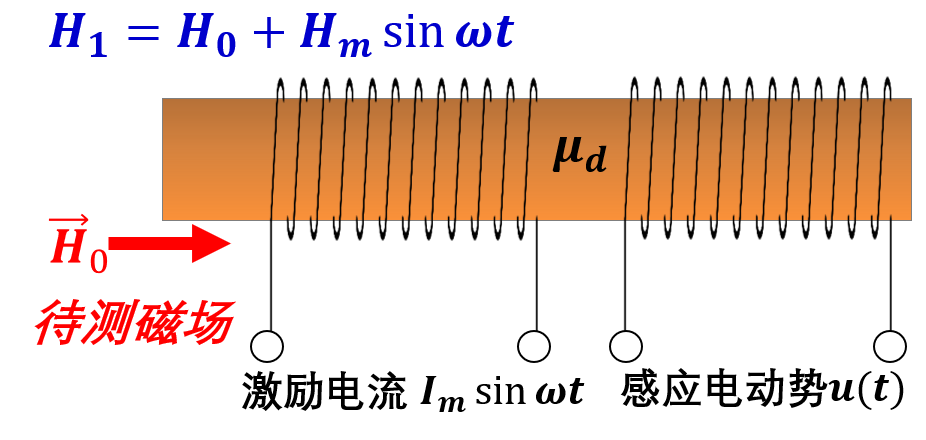
\includegraphics[width=11.5cm]{PICS/fluxgate.png}%插入图片。图片位置为相对主文件的相对路径,或绝对路径。句柄width为图片宽度。
\caption{磁通门磁强计的基本结构}%图注
\end{figure}%插图环境结束。
在文档的任意地方,你都可以利用$\backslash ref\{$图片的特定标签$\}$来跳转到标签指示的图片处。同理,表格,公式等也可以用此方法。后文细讲。
\reposec{如何插入公式}
插入公式有三类办法。
\reposubsec{单行公式}
顾名思义,单行公式只适用于仅有一行的公式。单行公式会整体居中,并在页面最右形成编号,例如:
\begin{equation}
1+1=2\label{eqn01}
\end{equation}
但也可以通过给单行公式加*号来取消编号。
\begin{equation*}
1+1=3
\end{equation*}
也可以自定义编号
\begin{equation}
1+1=11\tag{99}
\end{equation}
公式编号可以被交叉引用$\backslash ref$命令查询到,但前提是先在对应的想要引用的公式后面加上$\backslash label$命令进行标注,例如式\ref{eqn01}中的写法。请参考源代码。但一切的交叉引用若要生效,xelatex编译命令至少执行两次。否则会显示两个问号。\par
同时,如果是方程组,虽然有多行,但应当只使用一个标号的情况,可以采用cases环境来编写,例如:
\begin{equation}
\begin{cases}
B_S &\to\ 0.2\sim0.3T,\\
W_H&\to\ 0,\\
\dfrac{B_R}{B_S}&\to\ 0.5;\\
H_C&\to\ 0,\\
\mu_{init}\ &\to\  max\ .
\end{cases}
\end{equation}
\reposubsec{多行公式}
多行公式与单行公式大体相同,上面说到的关于编号、cases等的用法也可以大致通用。只是,多行公式涉及一个对齐的问题。多行公式的每行之间以$\&$这个符号的位置对齐,这个符号并不显示。在对其的前提下,整体再居中。例如下面的几行,以等于号对齐。其实,在上面的cases环境中,我们已经用到了$\&$来帮助对齐了。\par
\begin{align}
\mu_d&=\frac{1}{\mu_0}\frac{dB}{dH_1}\\
&=\frac{1}{\mu_0}\left(a-\frac{3}{2}bH_m^2+\frac{3}{2}bH_m^2\cos (2\omega t)\right)
\end{align}
\reposubsec{行内公式}
刚才的两种公式都是行间公式,每次进入公式环境,LaTeX都会自动新起一行。但如果想要在文字的中间插入公式或特殊符号,就需要行内公式了。很简单,用两个美元符号,将要写的公式放在中间即可,比如$\$\backslash mu\_d=\backslash frac\{1\}\{\backslash mu\_0\}\backslash frac\{dB\}\{dH\_1\}\$$可以表示$\mu_d=\frac{1}{\mu_0}\frac{dB}{dH_1}$作为行内公式。作为行内公式,latex真的比word排版得好看的多。
\reposec{如何插入表格}
表格是一个很复杂的东西,latex能插入的表格总的来说是比较简单的,很难实现复杂的效果,不建议拿LaTeX当MS Office Excel使用。我这里只提供一个简单的例子。最好还是参考文件夹里附送的《102分钟掌握LaTeX》的文档来搭建表格。
\vspace{0.3cm}
\renewcommand\arraystretch{1.7}
\begin{center}
\begin{tabular}{>{\raggedleft\arraybackslash}p{110pt}|>{\raggedright\arraybackslash}p{165pt}}
	\hline
	2022年2月至5月&完成非晶磁通门原型机搭建\\
	\hline
	2022年4月至9月&继续探索进一步噪声压制手段\\
	\hline
	2022年6月至7月&形成成果并发表\\
	\hline
	2022年1月前&完成毕业论文和学位答辩\\
	\hline
\end{tabular}
\end{center}
\vspace{0.3cm}\par
解释一下上方的各个语句,请结合源代码查看。\par
$\backslash vspace\{\}$命令是垂直空白距离,即Verticle Space。\par
$\backslash renewcommand\backslash arraystretch\{\}$命令改动了array宏包默认的表格的行高。默认为1倍行距。花括号内填充的数字即为行距的倍数。\par
$\backslash begin\{center\}$居中环境开始,与后方的$\backslash end\{center\}$(居中环境结束)成对出现,作用是将表格整体居中。\par
$\backslash begin\{tabular\}$表格环境开始。接下来的花括号内都是表格的格式和修饰项。具体还是应该去看教程。我在这里也简单讲一下。
\begin{enumerate}
\item $>$是arrary宏包提供的功能,用于在表格定义参数的这个花括号内,直接对每一列的属性进行设置,避免单独设置的麻烦。
\item 第一列:
\begin{enumerate}
\item $\backslash raggedleft$,直译为左边参差不齐,也即是文字居右。
\item $\backslash arraybackslash$,使用了前一个标志$\backslash raggedleft$之后,表格的换行符$\backslash\backslash$可能会出错或失效,因此要加上这个标志,防止编译出错。
\item $p\{110pt\}$表格格式声明符,注意最前面并没有反斜线。这一个标志的意思是,表格为固定列宽度(p)110磅(pt)。除了p之外,还有\textit{l, c, r}可以用,分别代表居左,居中,居右。但是注意,后三种参数不能强制规定列宽,也不能用$\backslash raggedleft$, $\backslash arraybackslash$这两个命令,列宽将会自动适应。我还是推荐使用$p\{\}$格式的表格,手动调节,会更美观一些。但一些较大的表格用p格式就可能太繁琐了。
\end{enumerate}
\item $|$竖线代表表格第一列和第二列之间的分界线为实线。如果不写这个竖线,则这两列之间没有分界线。但其他设置不变。同理,你可以看到由于第一列之前、最后一列之后没有写这个符号,所以表格最左边和最右边都没有边框线。
\item $>$同上。
\item $\backslash raggedright$,同理,直译为右边参差不齐,也即是文字居左。除此之外,你也可以用$\backslash centering$来居中。
\item $\backslash arraybackslash$,同上。
\item $p\{165pt\}$同上,但固定列宽为165磅。
\end{enumerate}\par
表格搭建完成,来看看内部的各个命令。\par
$\backslash hline$,即\textit{horizontal line},水平线。可以看作是行间分界线。\par
$\&$,对齐符号,在表格环境里就是每列之间分界的位置。\par
$\backslash\backslash$换行符号。\par
想要深入了解,去看教程。\par


\reposec{如何插入代码块,列表,摘要等特殊环境}
十分简单,不细讲了,详见教程第三章第五节。即21页开始的部分。
\reposec{如何引用参考文献}
在文章中插入参考文献有很多讲究。但是在开题,中期报告,或者我们日常写作论文的过程中,如果要使用这套模板,基本上只有三种模式以及一项前提。我现在手把手来教你。\par
\reposubsec{将参考文献加入数据库}
譬如说,你现在想要引用一篇文献,名字叫\ \textit{Orthogonal fluxgate magnetometers}\ 这篇文章的作者是M. Butta,发表于2017年。这篇文章如何下载当然大家是各显神通了。但现在我们需要去获得他的引用信息。\par
首先我们打开Google Scholar,找到这篇文章,并确认无误,如图\ref{fig01}。你也可以用别的手段,百度学术,Bing学术,基本上都有类似的操作可以实现。你也可以用Google Scholar的镜像站。\par
\begin{figure}[H]
\label{fig01}
\centering
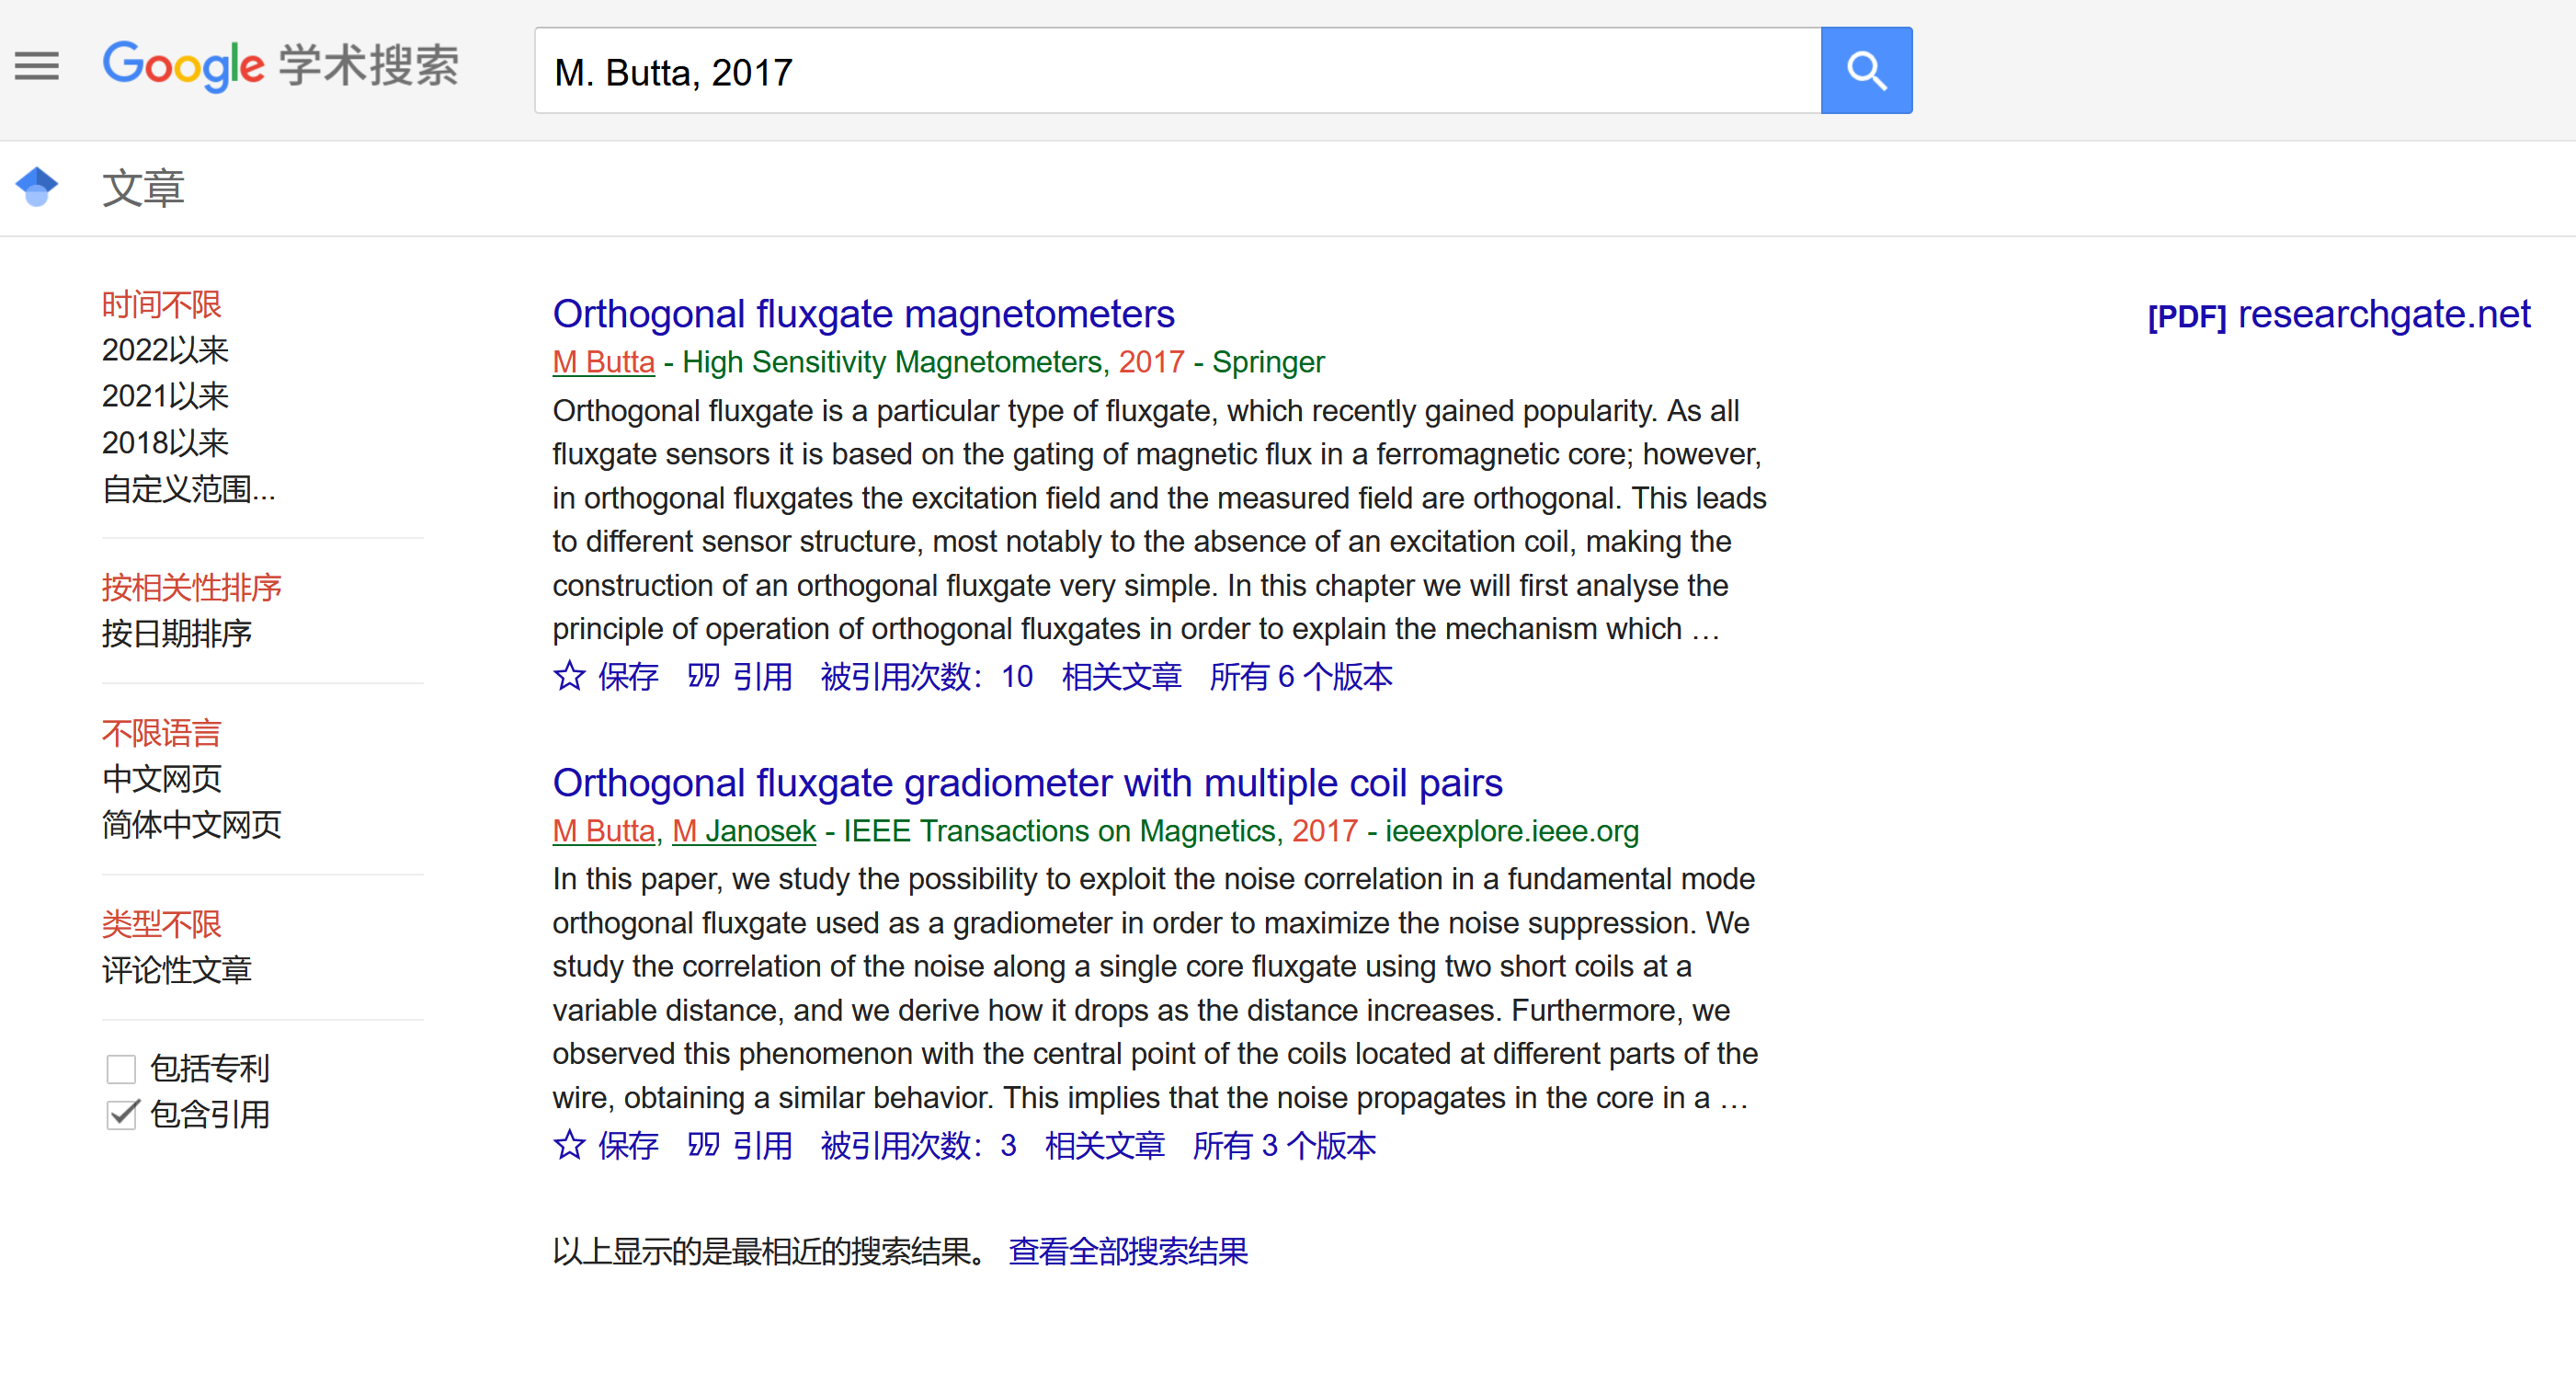
\includegraphics[width=11.5cm]{PICS/Cite1.png}
\caption{在谷歌学术上找到这篇文章}
\end{figure}\par
随后点击“引用”。
\begin{figure}[H]
\label{fig02}
\centering
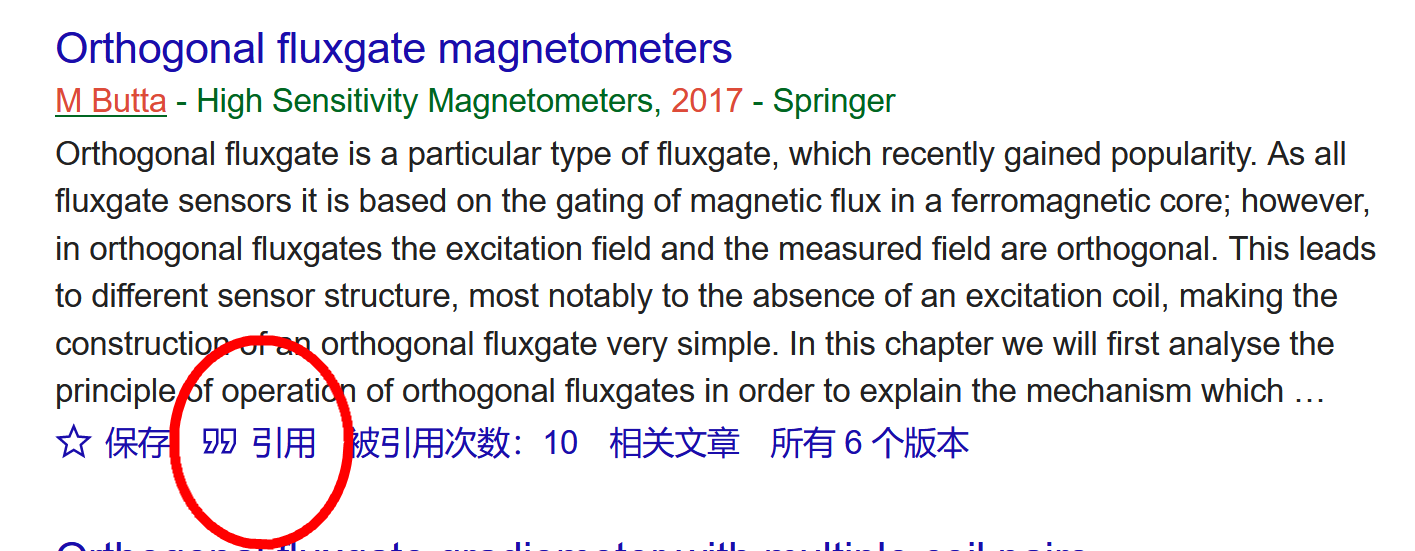
\includegraphics[width=8cm]{PICS/Cite2.png}
\caption{红圈里的引用点击一下}
\end{figure}\par
在弹出窗口里选择“BibTex”。
\begin{figure}[H]
\label{fig03}
\centering
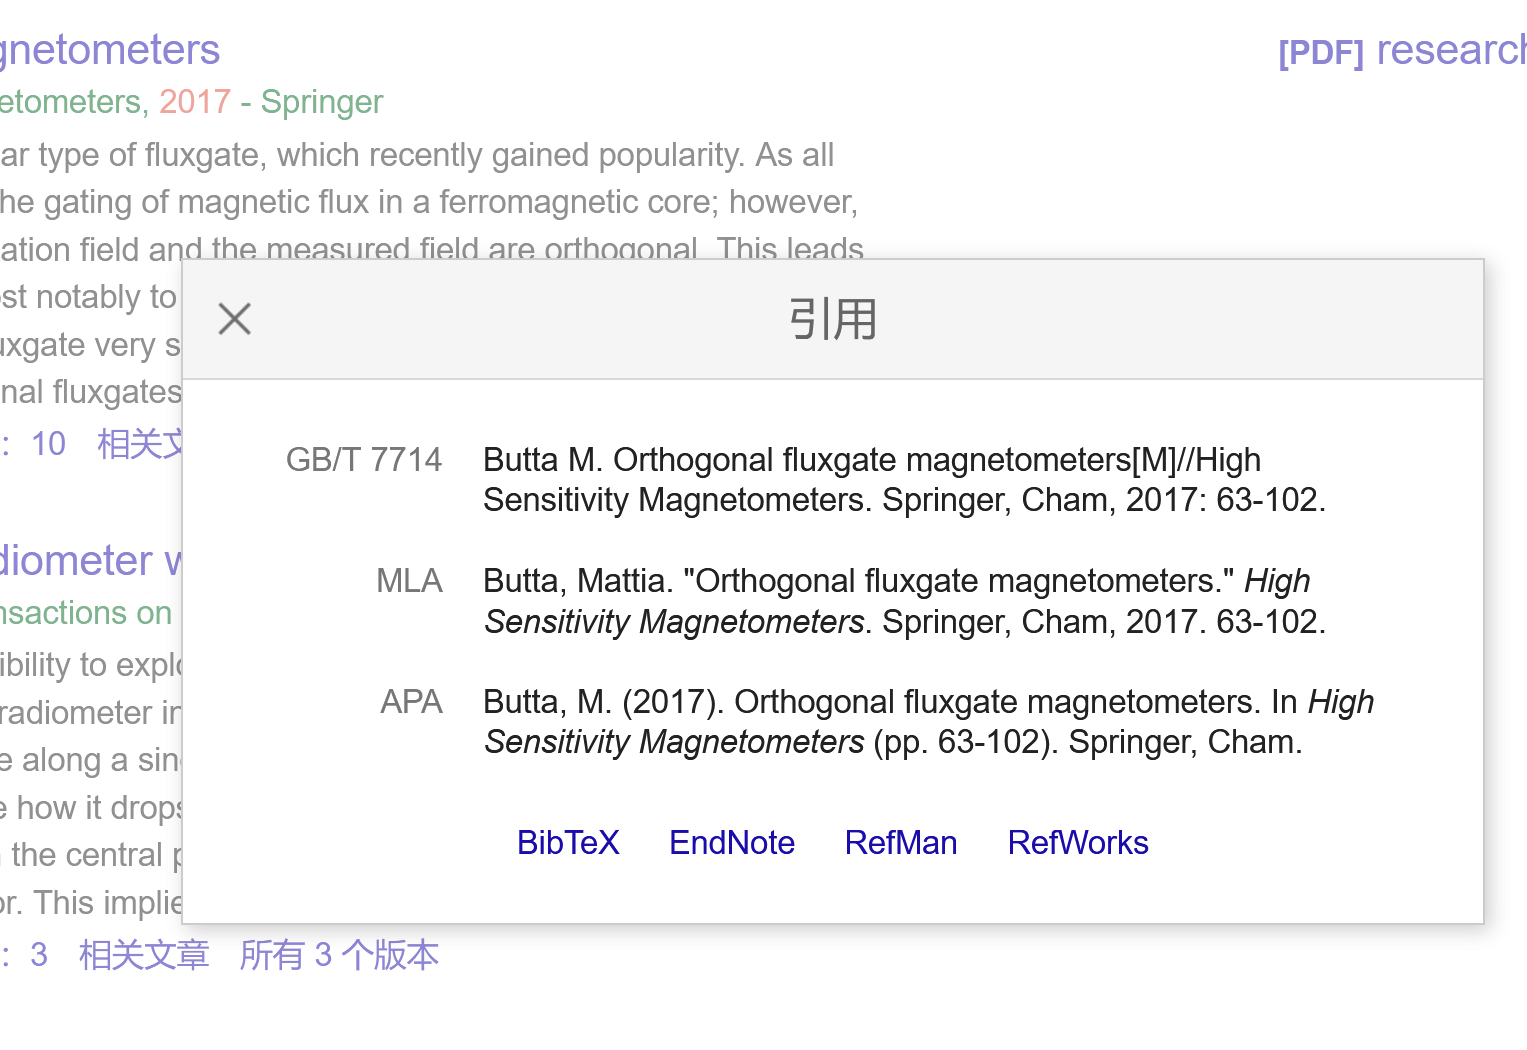
\includegraphics[width=8cm]{PICS/Cite3.png}
\caption{左下角的BibTex}
\end{figure}\par
然后会弹出一个窗口,里面有这样一些内容。
\begin{figure}[H]
\label{fig04}
\centering
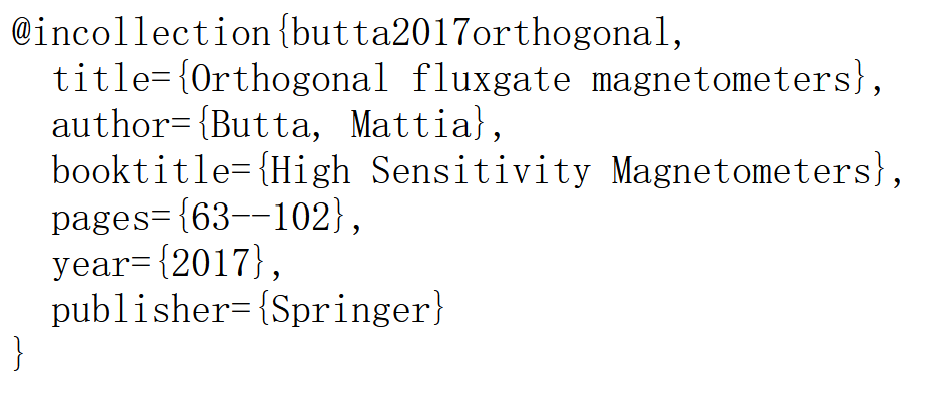
\includegraphics[width=8cm]{PICS/Cite4.png}
\caption{BibTex的全部信息。一般至少包括了题目,作者,年份,杂志(书籍),出版商等。有些还有DOI号,页码,网页链接等。不同的文献类别包含的基本信息也会不同,比如这篇是incollection,属于论文集的一部分。一般的文章是article,还有书籍book。详见教程。}
\end{figure}\par
全选并复制这些内容,粘贴进一个空白的txt文档中,例如\textit{testRef.txt},并另存为\textit{testRef.bib}。值得注意的是,这是一个文本文档,所以编码模式很重要。如果你的参考文献中只有英文,那么可以忽略。但如果你的参考文献中还含有中日韩语,西里尔文,拉丁文,希腊文的话,一定要注意编码模式,ANSI或GB2312可能会导致一系列的报错,尤其是会导致中日韩文出现乱码。另存为的时候一定要注意编码模式设置为UTF-8。具体如何设置请自行百度。
\begin{figure}[H]
\label{fig05}
\centering
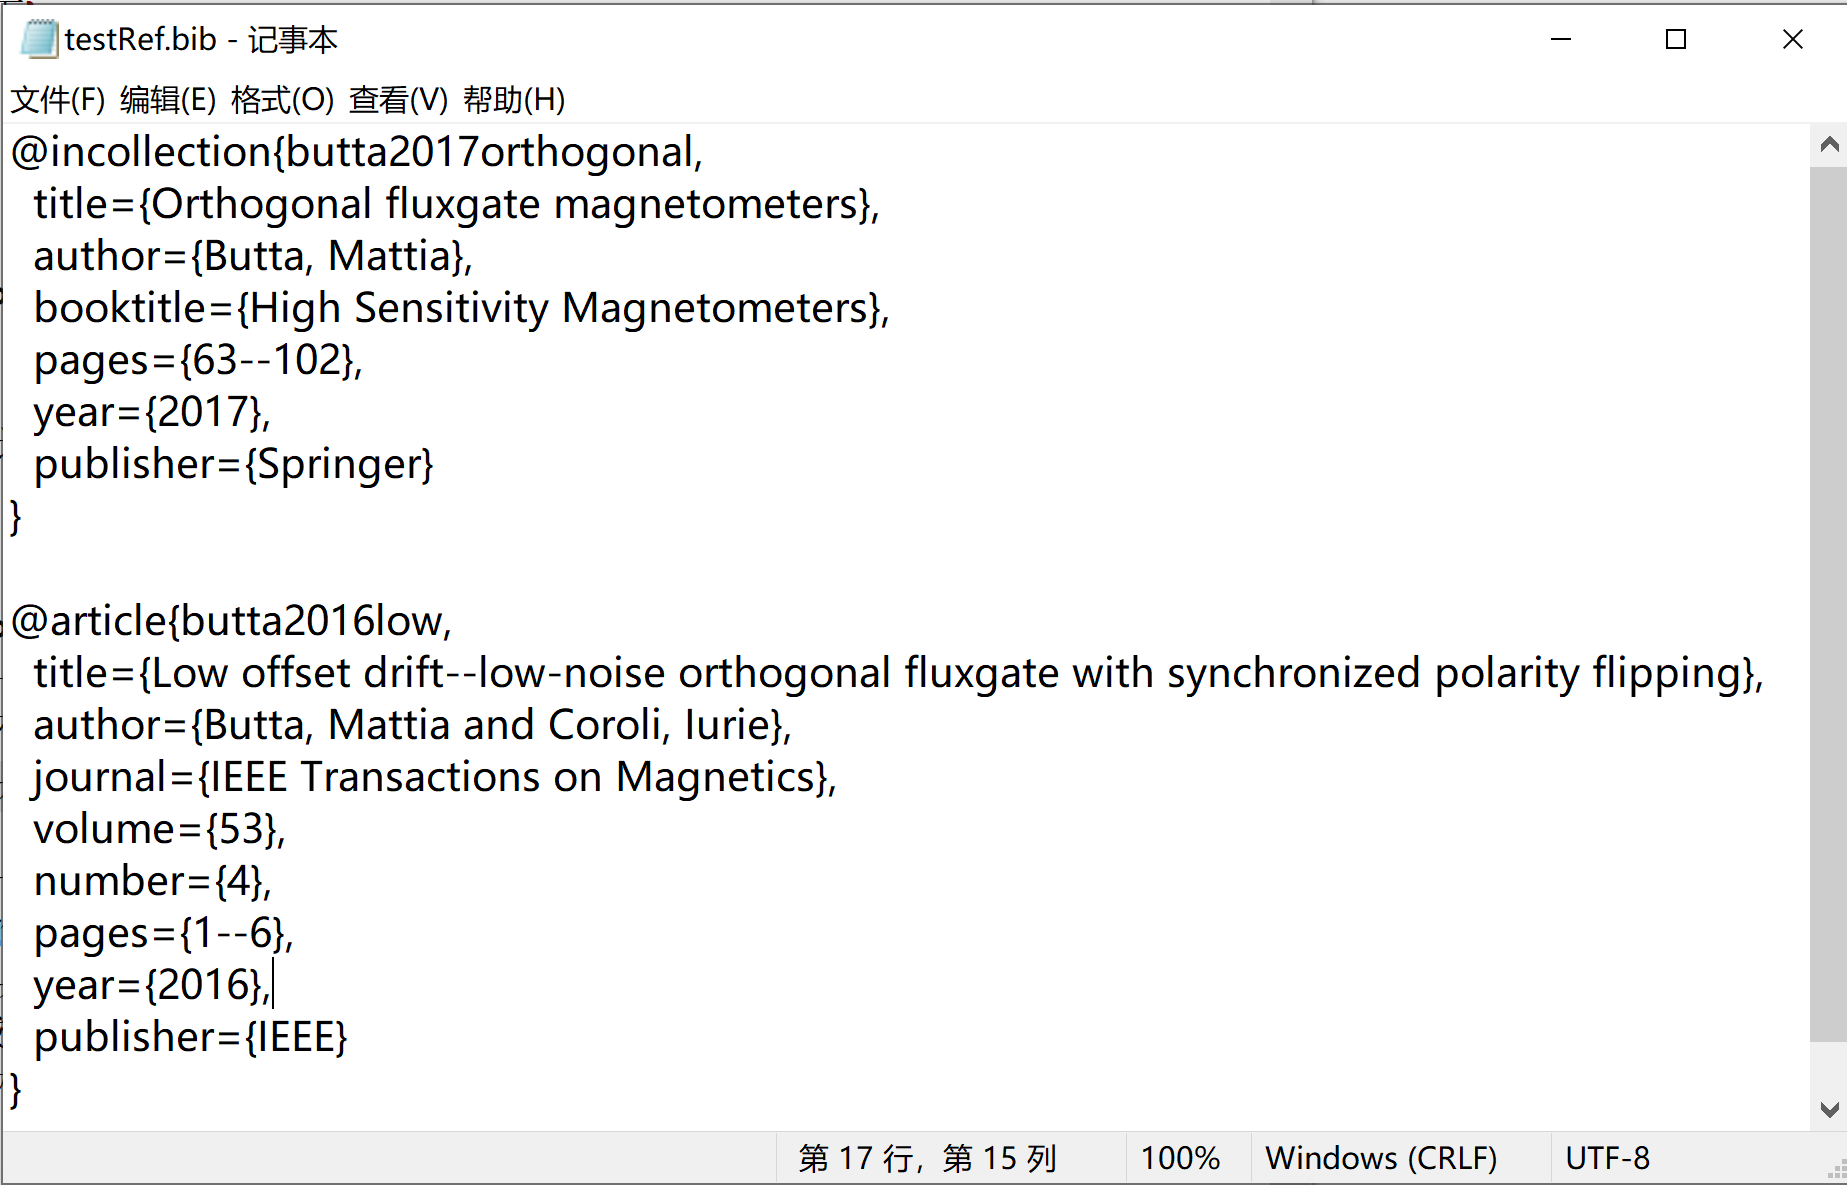
\includegraphics[width=9cm]{PICS/Cite5.png}
\caption{Bib数据库}
\end{figure}\par
注意,可以用一个Bib文件来容纳所有用到的或者没用到的参考文献。没用到的参考文献就算出现在了Bib文件里,如果文章中没有引用,也不会出现在最后生成的论文参考文献列表中。\par
你可以一边写论文,一边把自己用到的参考文献扔进这个库里。也可以从EndNote里批量导出Bib。Bib文件中的顺序无关紧要。另,Bib其实是bibliography的缩写,是参考文献的学名,意为目录学,参考书目,文献学,索引。\par
现在,你只要记忆如图\ref{fig06}红框圈出来的这个关键字,就可以在后面的教程中引用这篇文献了。\par
\begin{figure}[H]
\label{fig06}
\centering
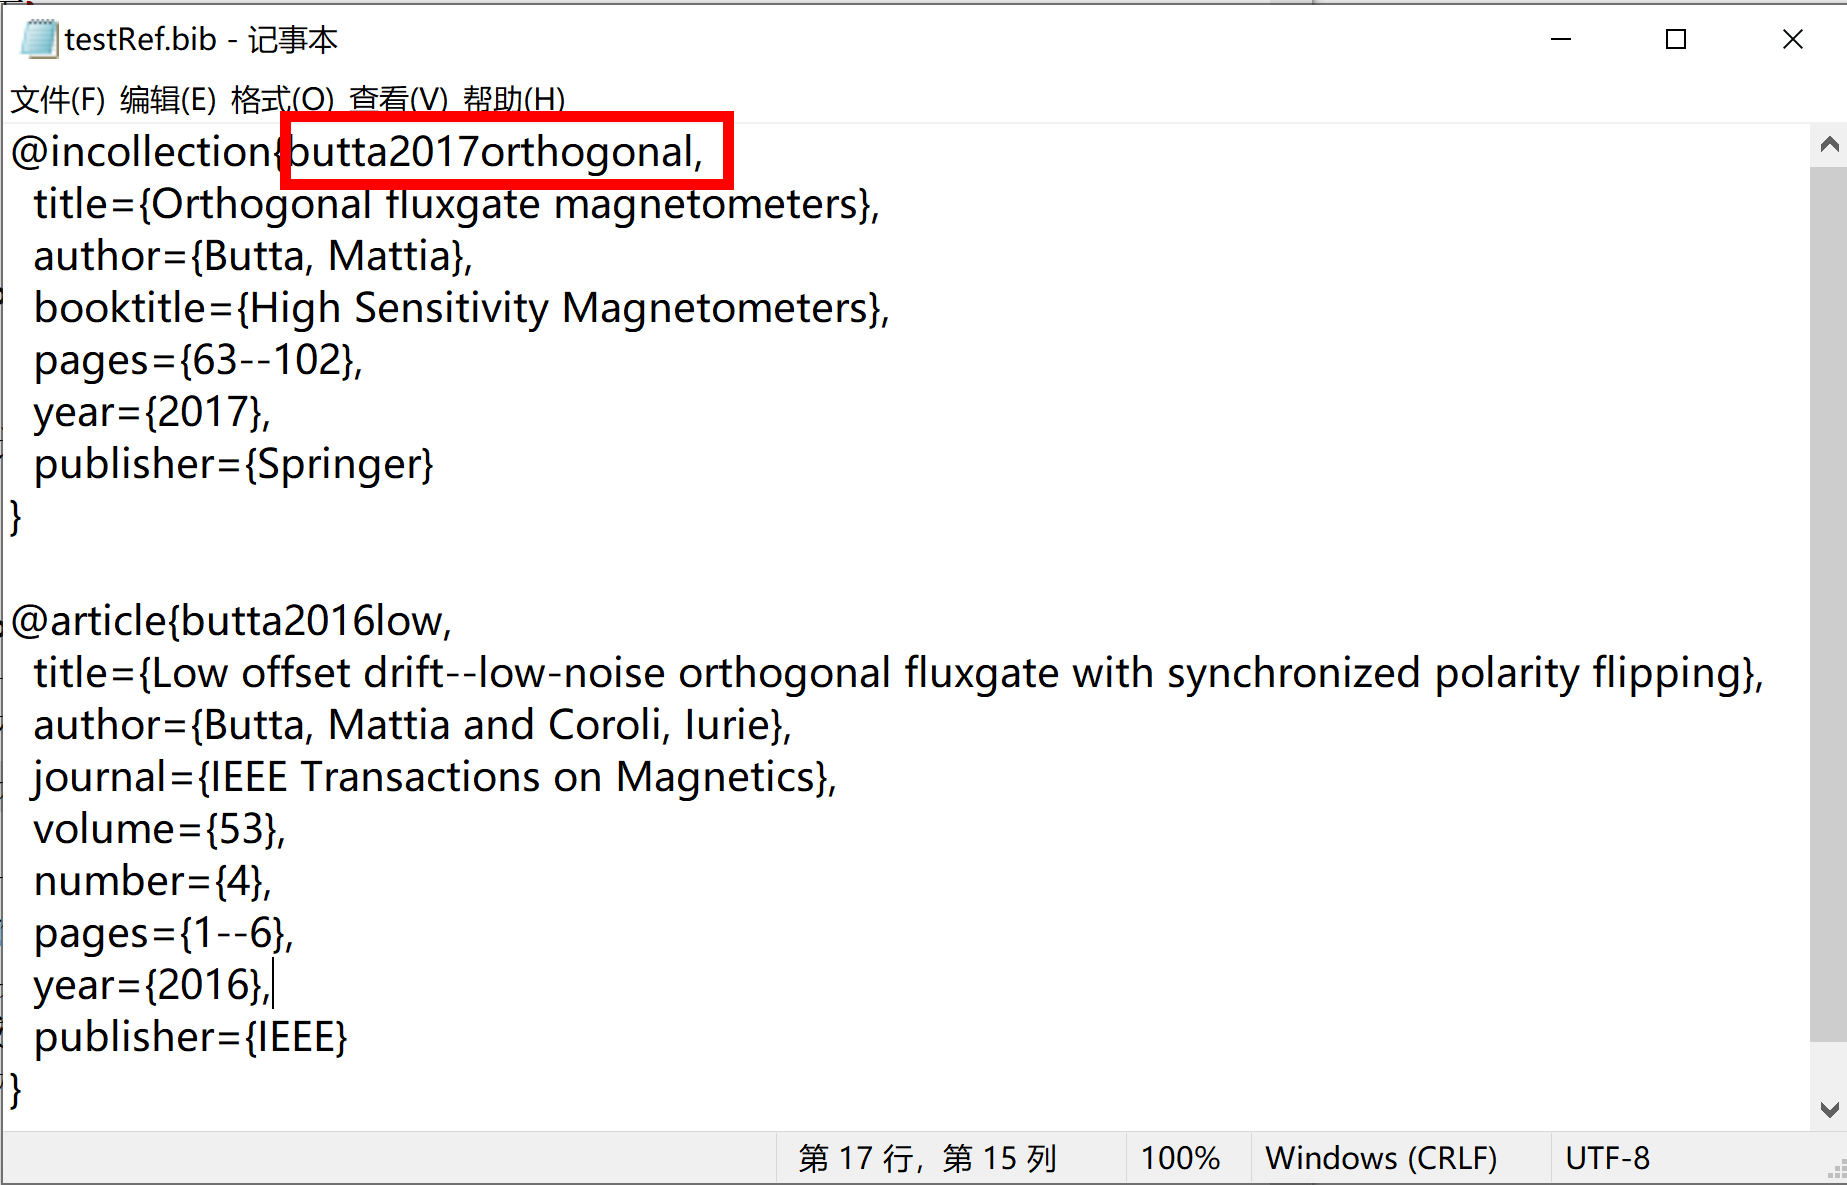
\includegraphics[width=9cm]{PICS/Cite6.png}
\caption{Bib关键字,注意,Bib库里绝不能存在重复的关键字,不然会报错。}
\end{figure}\par
\reposubsec{人名,时间都在括号里的完整引用}
当我们想要获得形如\citep{butta2017orthogonal}这样的参考文献样式,则你只需要在相应的位置使用$\backslash citep\{butta2017orthogonal\}$这个命令标志即可。其中的\textit{butta2017orthogonal}就是我前面说到的参考文献的关键字。只要这个关键字所代表的文献在你的参考文献库中,就可以成功引用。在文中你可以多次引用同一篇文献,参考文献列表只会出现一次。\par
这个命令可以同时写好几篇参考文献,会自动并列放好,例如:\citep{Yuan2020Graphene, butta2017orthogonal},或者同一个作者的多篇文章:\citep{butta2017orthogonal, butta2012orthogonal}。注意,多篇文献的关键字之间用西文的逗号分割,不要用中文逗号!\par
\reposubsec{人名在括号外,时间在括号里的引用}
当我们想要获得形如:\ \ \textit{在非晶磁强计领域,\citet{butta2017orthogonal}做出了重大突破}\ \ 这样的参考文献引用样式时,只需要在相应位置使用$\backslash citet\{butta2017orthogonal\}$这个命令标志即可。注意,这个参考文献样式已经自带了人名,所以你不需要再写一遍人名了。如果有多名作者,名字后面会自动带上et al.。并且显然,同一个作者的多篇文章\citet{butta2017orthogonal, butta2012orthogonal}的形式也可以正确表示。\par
\reposubsec{非引用参考文献}
有些参考文献对于这篇文章很重要,但是你却找不到恰当的地方进行引用,那么你可以考虑非引用参考文献。这种引用形式不会出现在正文中,但却会出现在参考文献列表中。相应的命令是例如:$\backslash nocite\{butta2016low\}$这样的语句。模板中,这样的参考文献统一写在了主文件Report.tex的正文部分最后。\par
\reposubsec{编译注意事项}
仅仅写了这些citep,citet或者nocite的引用项,并不会在文章最后生成引用文献列表。这需要你在需要插入参考文献的位置,添加一句话。$\backslash bibliography\{testRef\}$,注意将testRef修改为你自己的Bib库的名字。这句话放在哪里,就会在那个地方生成参考文献。\par
另外,为了使参考文献的数据库与文中的参考文献链接起来,并生成参考文献列表和交叉引用的链接,我们需要{\Large{\color{red}先跑一遍XeLaTeX编译,然后再跑一遍BibTex编译,然后再连续跑两遍XeLaTeX编译}}。没有别的捷径!
\reposec{其它杂项}
生成的pdf文档不要直接在TexWork软件里打印,最好用MS Edge浏览器或其他浏览器打开,再打印。在Tex的GUI里打印,有可能会把超链接和交叉引用上那个方框也打印出来,就很糟糕了。包括Okular这个PDF浏览器也不行。\par
暂时想不到更多的需要注意的点。如果你有不了解的,还可以直接询问作者。\faPhone: +86-18810909715。\faEnvelope :\href{mailto:yuankx13@mail.ustc.edu.cn}{yuankx13@mail.ustc.edu.cn}。\faQq : 870218493。
%\input{./Chapters/chapter01}
%\input{./Chapters/chapter02}

%%%%%%%%%%%%%%%%%%%%%%%%%%%%%%%%%%%
%citation part, generate the bibliography
%%%%%%%%%%%%%%%%%%%%%%%%%%%%%%%%%%%

%Those you readed and used, but not cited, put them here and enable the `nocite'
\nocite{butta2016low}%未在文中出现,但确实重要的参考文献
\lastthing
\newpage%更换空白页
\addcontentsline{toc}{section}{\Xiaosan\textbf{参考文献}}%生成参考文献的目录项,如果不需要目录,记得注释掉这句话。
\bibliography{testRef}%注意修改成你自己的Bib库的名字
\end{document}%z这一语句之后的信息,理论上都不会生效。但写错了会报错。